\chapter{高可用在线服务在竞价云上的轻量级暖备方案}
\label{cha:gemini}

\section{本章概述}
\label{sec:gemini_intro}
随着IT信息技术的迅猛发展,人类的日常工作生活中已经习惯了无处不在、无所不能的互联网服务。很多互联网业务都要求24x7(每天每刻在线)提供服务。同时,这些互联网服务还要求快速响应用户请求,例如:互联网视频直播,电子购物网站,社交网站等。这进一步要求后端服务(如:数据库服务或对象存储服务)的高可用性。正如Amazon EC2云平台的帮助文档 \cite{SI:2014} 中所建议的,竞价计算实例适合时间灵活(Time Flexible)及可容忍中断(Interruption Tolerant)的任务。传统观念也认为要求高可用性的服务应该托管在专用服务器或可靠的虚拟机实例上,而不是使用竞价计算实例。许多前人的研究工作 \cite{chohan2010see, Liu:2011:CMC:2170444.2170450, song2012optimal, Yi:2010:RCS:1844768.1845343, Andrzejak:2010:DMC:1906481.1906533} 持相同的观点和顾虑,聚焦于如何修改已有的计算框架适配竞价实例潜在的被回收风险。这些计算框架通过重执行、任务检查点、批处理作业负载迁移等技术手段来容忍竞价实例失效。然而,成本下降带来的巨大经济利益驱动着使用竞价计算实例提供在线服务的研究工作。进来,He等人的研究已经表明使用竞价实例提供互联网服务是可行的。他们的方法基于嵌套虚拟化技术和多种先进的虚拟机迁移技术。

然而上述使用竞价实例提供在线服务的研究工作有很大的局限性。基于虚拟机迁移技术的方法 \cite{He:2015:CCH:2749246.2749275} 面临着强制性的在线服务不可用。这类不可用问题出现在云平台回收竞价节点的过程中。由于新的虚拟机实例启动和虚拟机迁移的时间通常超过云平台的告警通知时间,竞价实例上托管的在线服务不得不忍受这期间的不可用。即使虚拟机的快照操作通过时间可控的内存检查点技术得以及时完成 \cite{Singh:2013:YEG:2482626.2482642},根据文献\cite{Hines:2009:PBL:1508293.1508301}的测试结果,虚拟机延迟恢复技术也不可避免地产生约20秒的服务停机时间。

除了强制性的不可用问题,性能也是在线服务提供商必须考虑的关键问题。更具体地说,在线服务性能的一个重要指标--响应时间对用户体验或者说服务质量(Quality of Service)是尤为关键的。然而,之前的研究工作只关注在线服务的可用性和成本,而忽视了服务的性能。出于对数据和内存检查点数据丢失的考虑,之前的方法选择使用持久化的网络接入存储卷EBS而放弃了高性能的本地存储卷Instace Store。然而,对于很多在线服务来说,服务性能的瓶颈就来自底层存储。此外,基于嵌套虚拟化和虚拟机迁移技术的方法 \cite{He:2015:CCH:2749246.2749275} 对于计算密集的服务带来了不可接受的性能开销。嵌套虚拟化技术在支撑互联网服务时至多带来50\%的性能开销 \cite{He:2015:CCH:2749246.2749275},对于一些计算密集型的测试集,性能开销高达68\% \cite{Williams:2012:XVO:2168836.2168849}。

本章重新审视并探讨了使用竞价实例提供高可用在线服务的问题。更进一步地,本章力求回答一个更有挑战性的问题:能否打破当前最先进的解决方案的局限性,使得使用竞价实例部署的在线服务同时实现高可用性、高性能、成本低廉?本章提出了一个全新的基于暖备和互备技术的解决方案并实现了一个原型工具Gemini。Gemini基于轻量级的服务迁移方法和综合考虑市场价格及其稳定性的智能可用区选择策略。这里,术语``暖备'' 不同于 ``冷备'' 和 ``热备''。暖备是指用作备援的虚拟机实例一直处于运行状态,但主备节点的状态不是实时同步的。互备是指两个节点互相作为对方的备援节点,形成一个互备对。在线服务提供商可以在这样的两个节点上运行同一服务的两个分片或是一个服务的不同组件。为使得这样一套机制正常运作,Gemini中包括三个不同的组成构件:一个部署于每个节点上的执行进程活迁移(Live Migration)磁盘同步任务的代理,一个控制服务迁移和维护暖备、互备状态的迁移控制器,以及一个申请或购买新的虚拟机计算实例的节点调度器。通过使用暖备技术,申请新虚拟计算实例和进行虚拟机快照的时间开销得以从服务迁移的关键路径中移除。因此,Gemini能够使用竞价实例提供可用性更高的在线服务。通过时间可控的异步磁盘镜像机制,Gemini可以在保证服务可用性的同时使用虚拟机实例的高性能本地存储得到数倍到数十倍于网络存储的I/O性能。通过改用轻量级的进程迁移技术,Gemini避免了嵌套虚拟化和虚拟机迁移带来的大量性能开销。
总的来说,本章的贡献主要包括:

\begin{enumerate}
\item 通过详细分析当前最先进的使用竞价实例提供高可用服务的解决方案,指出了其阻碍使用竞价实例部署高可用在线服务的主要缺陷是强制性的服务不可用问题和较低的性能。
\item 提出了新的使用竞价实例提供在线服务的方法和框架Gemini。Gemini基于轻量级迁移和暖备、互备技术,能够智能选择价格稳定区域申请竞价节点。
\item 实现了一个Gemini的原型系统以验证其有效性。评测结果显示在相近的成本下相比之前的基于嵌套虚拟化和虚拟机的技术获得了显著的服务可用性级别和性能提升。
\end{enumerate}

\section{现有系统局限性}
\label{sec:gemini_challenges}
为了使用竞价实例提供在线服务,之前的基于嵌套虚拟化和虚拟机迁移技术的方法\cite{He:2015:CCH:2749246.2749275}本质上是一个冷备方案。在面临强制性服务迁移的场景下,备援节点需要在告警时间内先启动然后恢复主节点的虚拟机状态。然而在Amazon EC2云平台上启动一个虚拟机实例的时间就接近甚至超过了竞价实例回收告警时间。根据对各个云平台虚拟机实例启动时间的全面调研 \cite{Mao:2012:PSV:2353730.2353859},Amazon EC云平台上按需计算实例使用一个默认Linux操作系统镜像的平均启动时间是96.9秒。随着系统镜像大小的增长,虚拟机实例的启动时间相应地线性增长。即使是一个1GB大小的Linux系统镜像,按需计算实例的启动时间也超过了目前两分钟的竞价实例回收告警时间。至于竞价实例的启动时间相对按需实例则表现的更加缓慢且差别更大,因为竞价实例的申请需要花费一段时间分配然后才能开始启动过程。因此,基于冷备的解决方案面对强制性的服务迁移状态有些微妙。无论虚拟机迁移的过程可以多么快的完成,如果备援节点的启动过程所需时间超过了回收告警时间则必然面临一段时间的服务不可用状态。这个关键的挑战在目前仍未解决。

另一个挑战是服务性能相关的。I/O密集的在线服务需要高性能的底层存储。如表 \ref{table:ec2storage} 所示,对于I/O密集的在线服务SSD实例存储(Instance Store)是理想的块存储设备,有着超高的性能和零额外成本。然而实例存储是暂时性的,只在其对应的虚拟机实例的生命周期内可用。使用DRBD复制数据到一个远程的镜像存储设备或是部署RAID1实时同步到一个持久化的EBS都能保证实例存储的数据持久化。但这样的数据复制机制由于网络或EBS存储的延迟和带宽问题使得SSD实例存储的性能大大降低,致使这样的数据复制毫无意义。对于OLTP(On Line Transaction Processing)这类需要高性能存储的在线服务,另一个选择是使用预留IOPS的SSD EBS。但SSD EBS预留的高IOPS需求大量成本,消除了性能提升和改进的意义。根据Amazon EBS的定价说明 \cite{EBSPricing:2015},一个预留了10000 IOPS,160 GB 大小的SSD EBS一个月的成本超出了拥有同样大小的SSD实例存储的 ``Linux c3.2xlarge'' 类型的按需实例价格的两倍多。如何持久化数据并同时保证SSD实例存储的高性能是一个有挑战的技术难题。
\begin{table*}
\centering
\caption{Amazon EC2 Storage Performance Details}
\label{table:ec2storage}
\begin{tabular}{c|ccc} \hline
Storage Type& Throughput (MB/s)& IOPS (4KB)\\ \hline
Ephemeral SSD & 733 & 100,000\\ \hline
Persistent SSD 1 & 160 & 10,000\\ \hline
Persistent SSD 2 & 320 & 20,000\\ \hline
Ephemeral HDD & 110 & 200 \\ \hline
Persistent HDD & 40 - 90 & 100\\ \hline
\end{tabular}
\end{table*}

另外,一个好的解决方案应避免引入过大的性能开销。因为对CPU、内存、网络、I/O带宽的占用可能导致在线服务性能的下降。这意味着我们需要更多的计算资源提供同样的在线服务。任何额外的成本支出减少了使用竞价实例带来的成本收益。例如:使用基于嵌套虚拟化的方法引入了大量的CPU开销,导致在线服务平均响应时间增加为原来的两倍。再者,采用虚拟机迁移技术来实现服务迁移也不够轻量级,迁移虚拟机操作系统的内存带来的时间开销是不必要的。

\section{Gemini系统设计与实现}
\label{sec-gemini}
Gemini着眼于前述的使用竞价实例提供在线服务面临的几个挑战。当前的解决方案 Cloud Scheduler \cite{He:2015:CCH:2749246.2749275} 主要采用了一个类似冷备的错误恢复机制。相比之下,Gemini使用了基于暖备的方法来解决 Cloud Scheduler 没有解决的问题。当竞价实例市场价格陡升超过用户出价时,使用该节点的在线服务不得不进行一次强制性的迁移。如图 \ref{fig:timeline1} 所示,在收到竞价实例回收告警时,Cloud Scheduler 选择请求一个按需实例并在该虚拟机实例启动后在其上恢复被回收竞价实例节点的状态。在Amazon EC2云平台,启动一个使用默认Linux操作系统镜像的按需实例所需时间变动很大。虽然平均启动时间是90 $\sim$ 100秒,但在一些测试中已经超过了两分钟的回收告警时间。并且,随着操作系统镜像大小的增加启动时间也线性的变长。因此,当竞价实例被回收后,新申请的计算实例可能仍处于启动过程中而不可用。在Cloud Scheduler的评测过程中也反映出了这个问题 \cite{He:2015:CCH:2749246.2749275}。使用暖备技术能改变这个状况,如图 \ref{fig:timeline2}所示,在收到回收告警的一刻起服务迁移就直接开始了。新请求的计算实例即使在竞价实例被回收之后启动也没有关系,在线服务可以在暖备节点上运行而不会不可用。在新请求的替代节点启动完成可用后,在线服务可以有计划地迁移过去。并且有了暖备节点,无需再从网络磁盘上恢复在线服务的状态。反之,Gemini可以通过活迁移技术大大消除虚拟机迁移过程中的冻结时间导致的服务不可用时间。虚拟机活迁移技术的冻结时间可以低至数十毫秒 \cite{Clark:2005:LMV:1251203.1251223}。
\begin{figure}
  \centering%
  \subcaptionbox{基于冷备的方法\label{fig:timeline1}}
    {
\includegraphics[width=1.0\textwidth]{timeline1}}%
  \\
  \vspace{5em}%
  \subcaptionbox{基于暖备的方法\label{fig:timeline2}}
      {
\includegraphics[width=1.0\textwidth]{timeline2}}
  \vspace{5em}%
  \caption{不同故障转移方法的在线服务迁移时间线}
  \label{fig:timeline}
\end{figure}

许多在线服务使用多层架构。例如:一个电子商务系统通常包括一个Web服务器层,一个有数据库服务器、广告服务器、邮件服务器等的中间层,一个负责仓储物流等商业应用的后端层。单层的服务也可能需要运行多个分片来扩展性能。因此,Gemini可以利用这个机会让这些节点互相作为备援组成互备对,而无需申请新的虚拟机实例作为备用节点。即使是一个单机运行的架构,启用一个额外的竞价实例作为备援节点以获得更好的可用性也是值得考虑的。为了避免竞价节点回收时的关联失效问题,Gemini必须保证主节点和备援节点在不同的可用区。除了利用已有节点组成互备对,出于减少在线服务性能开销的考虑,另外一种方式是使用专门的备援节点。然而,不像热备在主备节点间实时复制操作,Gemini基于暖备的设计只有很小的性能开销。再者,这种类似备用服务器池方法需要保证备用服务器的可靠性,而Gemini采用互备对的方式能均衡地在所有服务器节点上分摊竞价实例的失效风险。
\begin{figure}[]
  \centering
  
\includegraphics[width=1.0\textwidth]{gemini}
  \caption{Gemini整体框架}
  \label{figure:gemini}
\end{figure}

Gemini的组成包括:一个Gemini代理,运行在每个虚拟机实例上执行服务迁移任务;两个组件,一个迁移控制器和一个虚拟机实例调度器。迁移控制器负责维护服务器节点间的互备对以及在竞价实例被回收时将备援节点切换为主节点。他需要同存在于每个节点上的Gemini代理通信,命令后者执行具体的迁移任务。后者则要负责磁盘镜像,和进程活迁移等任务。实例调度器负责购买或申请新的虚拟机实例以替换被回收的竞价实例或是更贵的按需实例。通过在多个市场间使用启发式的可用区选择策略,实例调度器试图同时保证高可用和成本节约。

\subsection{Gemini代理}
不像冷备的方式在主节点失效后才启动,也不像热备的方式实时地在主备之间复制所有操作,暖备方式能实现接近瞬时的恢复速度,同时也避免了实时复制操作的巨大性能开销。在暖备架构中,Gemini能够利用竞价实例的回收告警安全地进行异步磁盘镜像。通过时间可控的同步机制可以保证没有数据状态丢失。图 \ref{figure:arch} 说明了暖备架构是如何工作的。其中 ``主节点'' 和 ``备节点'' 是逻辑上的。每个节点都是主节点也是所处互备对中另一个节点的备节点。主节点在收到回收告警时可以发起一次到备援节点的服务迁移。暂存的实例存储上的磁盘更新被不断地、定期地同步到持久化的EBS上。
\begin{figure}
  \centering
  
\includegraphics[width=1.0\textwidth]{arch}
  \caption{暖备架构}
  \label{figure:arch}
\end{figure}

之前的解决方案\cite{He:2015:CCH:2749246.2749275} 依赖于嵌套虚拟化技术 \cite{Williams:2012:XVO:2168836.2168849} 和多种虚拟机迁移技术 \cite{Singh:2013:YEG:2482626.2482642, Hines:2009:PBL:1508293.1508301} 实现服务迁移。然而,XenBlanket,云平台上的嵌套虚拟化实现对于CPU密集型任务负载性能开销巨大。由于没有底层虚拟机管理程序(Hypervisor)的硬件虚拟化支持,XenBlanket无法实现像Turtles Project \cite{Ben-Yehuda:2010:TPD:1924943.1924973} 一样实现低开销的嵌套虚拟化。事实上,引入嵌套虚拟化是为了能够在云平台使用虚拟机迁移的技术手段。与之不同的是,Gemini另辟蹊径地选择了CRIU \cite{CRIU:2016},一个更轻量级的进程迁移方法实现服务迁移。因此,所有嵌套虚拟化带来的性能开销都不复存在。而且由于迁移力度从操作系统级别变成了进程级别,迁移过程中大量不必要的内存页传输也得以减少。更为重要的是,暖备的架构配置使得Gemini可以在竞价实例被回收时直接进行活迁移而不必在服务运行中定期保存内存检查点。

虽然利用竞价实例被回收的告警特性,服务进程的磁盘数据复制可以异步地进行,Gemini仍需保证在告警时间内可以完成同步操作。因此,为了保证不会发生数据状态丢失,Gemini必须实现过时数据量可控的磁盘同步机制。

假设可用于脏数据复制的网络或磁盘带宽是 $B$ ,告警时间是 $T$,Gemini代理通过控制脏数据量不超过 $B \cdot T$ 实现服务迁移时间可控。如果脏数据的量超过了这个限制,数据复制必须切换为同步模式。在一个实时同步模式下,在远程的副本操作返回前磁盘写操作将被阻塞。为阻止同步带来的性能严重下降,Gemini设置了一个小于脏数据量上限的数据复制阀值。当数据更新的大小超过这个阀值时,Gemini代理开始进行数据复制直至脏数据量低于这个阀值。这里,必须注意的是虚拟机实例的网络带宽是活迁移和磁盘镜像所需网络带宽之和的上限。

因为在当前云平台的配置中EBS是一个网络存储,实际上没有必要浪费主备节点的网络带宽传输磁盘更新到备节点。Gemini直接将逻辑上属于备节点的网络存储EBS挂载到主节点上,当发生服务迁移时,在重新挂载到备援节点上。因此,磁盘镜像工作可以完全在主节点一端进行,只消耗主节点的网络带宽。对于磁盘镜像,DRBD \cite{DRBD:2015} 是一个高可用(HA)集群中常用的主备节点间的磁盘镜像工作,它类似于通过网络传输的RAID-1。异步地磁盘镜像也可以通过一个软件RAID实现,Linux md \cite{Linux_md:2016} 的``write-mostly''特性实现。这些方法对于各个类型的磁盘I/O来说是通用的。本质上,暂存的SSD实例存储扮演了持久化的EBS的缓存设备的角色,消除了巨大的访问延迟。这里,Gemini使用Bcache \cite{Bcache:2016},一个块设备层的缓存,完成磁盘镜像的任务。通过限制缓存脏数据的比例,Gemini确保了磁盘镜像一直是时间可控的。通过调节后台写回速率,网络带宽的占用也得以平滑。

为近一步优化网络带宽占用,一些更有针对性的技术可以加以应用,如:Rsync \cite{Rsync:2016}。另外,Amazon EC2云平台提供EBS优化(EBS-optimized)的虚拟机实例。这样的虚拟机实例拥有提供给EBS I/O的额外专用网络带宽。使用这样的虚拟机实例可以消除EBS I/O对虚拟机实例网络带宽的消耗。但不是所有类型的虚拟机实例都支持EBS优化的特性。

\subsection{迁移控制器}
迁移控制器的任务是通过维护互备对保证服务的可用性。通过周期性地检查竞价实例的元数据,迁移控制器可以监控各个竞价实例的回收告警消息。当一个竞价实例将要被回收时,迁移控制器调用该节点上的Gemini代理发起服务进程的活迁移到其备援节点。作为存储备份的镜像EBS也需要被配置和挂载到备用节点上,迁移控制器还需要重新分配对外提供服务的Elastic IP地址到备援节点。服务的高可用(HA)机制降级为冷备配置,类似于之前的解决方案 \cite{He:2015:CCH:2749246.2749275}。作为一个备援节点,如果收到回收告警消息,其对应的主节点同样需要进行可用性配置回退。这些状态转移如图所示。当处在冷备状态下时,活着的节点需要做内存检查点。迁移控制器将强制服务使用EBS作为主存储设备,并将内存检查点数据存储在EBS上。在我们的实验中,磁盘镜像配置无需作出改变。
\begin{figure}[]
  \centering
  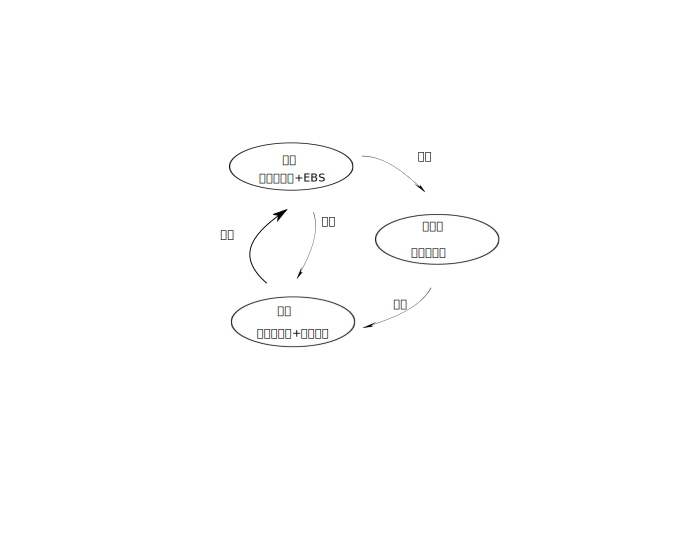
\includegraphics[width=1.0\textwidth]{states}
  \caption{在线服务状态转移图}
  \label{figure:states}
\end{figure}

当一个申请的竞价实例可用时,迁移控制器应该平滑地将在线服务恢复到正常的暖备状态配置。作为一个服务的备援节点,新加入的竞价实例只需简单的设置为所属服务中对应主节点的备援角色,迁移控制器还需将服务的主节点切换回暖备状态。作为一个服务的主节点,其所属的在线服务应通过进程活迁移转移到该节点,然后服务的暖备互备配置将得以恢复。这个新的主节点需要重新挂载用于持久化数据的EBS,将自身暂存的实例存储作为缓存设备。SSD实例存储同持久化的EBS形成时间可控的异步镜像配置。在线服务的IP地址也要分配给这个新的虚拟机实例。

当一个购买的按需实例启动完成时,作为一个服务的备援节点所需操作和竞价实例是相同的。作为一个服务的主节点,用于持久化数据的EBS被挂载后不再配置为时间可控的异步镜像方式。SSD实例存储中的脏数据比例不再受限制,写回(Writeback)持久化的EBS设备的操作被挂起。然后在线服务在该节点上恢复并进入没有备援节点的状态。在线服务可能过一段时间后需要从按需实例迁移回竞价实例。这种情况下,挂起的磁盘镜像要先恢复。在Gemini代理完成SSD实例存储同持久化EBS的同步工作后,再开始进行进程活迁移。由于没有时间上的限制,所有这些在线服务潜在的迁移过程相比强制性迁移都容易完成。

\subsection{虚拟机实例调度器}
当一个竞价实例被云平台回收时,虚拟机实例调度器将申请新的计算实例替换掉失效的节点。虚拟机实例调度器的任务是在众多可用区中申请一个竞价实例或购买一个按需实例。获取新的计算实例的策略应同时考虑成本效率和服务可用性两个因素。除了在被动的情况下获取新的计算实例,虚拟机实例调度器也会出于成本优化的考虑主动在竞价实例和按需实例间切换。

Cloud Schduler \cite{He:2015:CCH:2749246.2749275} 提出了两个获取竞价实例的策略:一个保守型(Reactive)策略是将竞价设为和按需实例相同的价格,一个主动型(Proactive)策略是将竞价设为高于按需实例的价格。保守型策略当竞价实例高于按需实例价格时需要进行服务的强制性迁移。主动型策略当竞价实例高于按需实例价格但没有超过设定的竞价情况下不会触发强制性竞价节点回收,可以主动地申请新的计算实例并将在线服务迁移到新的节点上。主动型策略能减少因竞价实例被回收而发生的强制性服务迁移次数,从而提升冷备配置下的服务可用性。由于Gemini已经解决了强制性的不可用问题,保守的计算实例调度可以带来比主动型策略更少的成本同时保证服务的高可用性。在可用区的选择上,Cloud Scheduler 采用了最为简单的贪心策略,即根据各个可用区竞价实例的市场价格选择最低者。Gemini则综合考虑了服务可用性和成本两个因素,针对价格和价格稳定性选择可用区。价格的波动可以用近期价格数据的标准差表示。价格的衡量可以使用近期价格数据的简单移动平均(Simple Moving Average),其计算方式为:
\begin{equation}
SMA = \frac{p_1 + p_2 + \cdots + p_n}{n}
\end{equation}

其中$p_i$表示最近第$i$个周期的竞价实例市场价格,$SMA$即为最近$n$个周期的竞价实例市场价格的简单移动平均值。

实例调度算法如图 \ref{figure:avz-selection-algo} 所示,首先列出所有竞价云可用区,排除掉互备对中另一个节点所在可用区以保证主节点和备援节点的失效独立性。然后计算各个可用区最近一段时间竞价实例市场价格的简单移动平均值 $SMA$ 和标准差 $\sigma$,移除标准差过大的可用区以保证价格平稳减少竞价实例被回收的情况。最后选出平均值最低的可用区,如果该可用区价格低于按需实例价格则申请竞价节点,否则在互备对中另一个节点所在可用购买按需节点。

\begin{figure}
\rule[-.2pt]{\textwidth}{0.9pt}
\textbf{Algorithm: SelectAvZ}

\rule[-.2pt]{\textwidth}{0.5pt}

\begin{algorithmic}[1]
\Require{$excluded$, $n$}
\Ensure{$selected$}

\State $zones\gets get\_availability\_zones()$
\ForAll{$zone \in zones$}
    \If{$zone = excluded$}
        \State $zones.remove(zone)$
    \EndIf
\EndFor
\ForAll{$zone \in zones$}
    \State $avg[zone]\gets SMA(zone.spot\_prices[1..n])$
\EndFor
\ForAll{$zone \in zones$}
    \State $sd[zone]\gets \sigma(zone.spot\_prices[1..n])$
\EndFor
\ForAll{$zone \in zones$}
    \If{$sd[zone] > ondemandPrice$}
        \State $avg.remove(zone)$
    \EndIf
\EndFor
\State $selected\gets min\_key(avg)$
\If{$get\_spot\_prices(selected) \not< ondemandPrice$}
    \State $selected\gets excluded$
\EndIf
\State \Return{$selected$}
\end{algorithmic}
\rule[-.2pt]{\textwidth}{0.8pt}
\caption{可用区选择算法}\label{figure:avz-selection-algo}
\end{figure}

在这个可用区选择算法中,竞价实例的市场价格标准差和移动平均值均使用最近 $n$ 个小时的价格历史数据计算得来。$n$ 值可以根据价格变化频率确定,默认值可设为一天时间(24小时)。可用区选择算法主要考虑备选可用区的价格稳定性和廉价性。通过设定一个标准差的阀值可以过滤不稳定的可用区,这里将该阀值设为按需实例价格。如果算法返回的可用区同互备对中另一个节点可用区相同则在该区购买按需实例,否则以按需实例价格作为竞价申请竞价实例。本章主要工作和重点在于使用轻量级暖备方案提升服务可用性和性能,在可用区选择算法上倾向于简单有效。因此,这里不再引入竞价实例市场价格的预测模型。在实际使用中,Gemini可以方便地替换虚拟机实例调度器,改用其他可用区选择算法。

此外,当前区域长时间没有可用的竞价实例时,虚拟机实例调度器可以选择发起一次区域切换。切换区域对于那些直接同用户交互的服务可能带来很大的响应请求延迟,对于这类服务最好保持在一个区域。另外需要注意的是,EIP是归属于一个区域的。在一个区域申请的EIP无法分配给另一个区域的计算实例。因此,直接同用户交互的服务如果切换区域。要求该服务有提供域名供用户访问,同时需要在切换区域后,更改DNS记录将域名映射到新的IP地址。同时在原IP所在节点上提供请求转发代理,直至DNS记录更新完成。

另外需要注意的是,由于一个区域的EBS卷无法在另一个区域使用,跨区域的互备是不可行的。因此,区域切换需要将运行在当前区域的服务整体迁移到其他区域以期使用成本更低的竞价实例。对于这种跨区域的虚拟机实例调度,选择区域的方法是基于选择可用区的策略的。具体算法如图 \ref{figure:region-selection-algo} 所示,首先对备选的区域使用可用区选择算法。不同之处是每个区域要选出两个可用区供获取主节点和备援节点,最后选择两个可用区移动平均价格之和最小的区域作为目标区域。在跨区迁移时,在线服务的EBS数据应首先拷贝到目标区域。然后,将在线服务的进程迁移到在该区域的获取的节点上。最后,迁移控制器要对暖备配置进行更新。

\begin{figure}
\rule[-.2pt]{\textwidth}{0.9pt}
\textbf{Algorithm: SelectRegion}

\rule[-.2pt]{\textwidth}{0.5pt}

\begin{algorithmic}[1]
\Require{$excluded$}
\Ensure{$selected$}

\State $regions\gets get\_regions()$
\ForAll{$region \in regions$}
    \If{$region = excluded $}
        \State $regions.remove(region)$
    \EndIf
\EndFor
\ForAll{$region \in regions$}
    \State $zoneA\gets region.selectAvZ(region.firstAvZ())$
    \State $zoneB\gets region.selectAvZ(zoneA)$
    \State $prices[region]\gets zoneA.spot\_price + zoneB.spot\_price$
\EndFor
\State $selected = min\_key(prices)$
\State \Return{$selected$}

\end{algorithmic}
\rule[-.2pt]{\textwidth}{0.8pt}
\caption{区域选择算法}\label{figure:region-selection-algo}
\end{figure}

\section{系统评测}
Gemini的原型实现基于CRIU,Bcache,和Amazon EC2 APIs。为全面有效的评价轻量级暖备方案的有效性,Gemini进行了一系列的实验。

首先,两个指标被分别用来确认和测量Gemini的两个组件。进程活迁移的时间对于Gemini来说是一个关键指标。它决定了使用活迁移技术在短的告警时间周期内完成在线服务迁移的可行性。另一个指标是在Gemini的时间可控的异步磁盘镜像配置下实例存储的I/O性能。它是I/O密集的在线服务潜在的性能瓶颈。

两个基准测试集,TPC-W\cite{TPCW:2014} 和 YCSB\cite{YCSB:2014} 负载下的 Mongodb\cite{Mongodb:2014},都被用于在线服务的性能评测。TPC-W是一个事务型的网上购物基准测试集,它有一个web服务器层处理顾客请求和一个数据库层维护购买、下订单等事物记录。MongoDB是一个非常流行的NoSQL数据库,它已经被广泛用于各种不同类型的在线服务。YCSB是一个用于比较各种不同的NoSQL数据库的相对性能的开源的规范和Java程序套件。

最后基于Amazon EC2公布的竞价实例市场价格历史数据,Gemini还进行了一些长期的在竞价云平台上的在线服务运行的仿真实验。这些实验评测了Gemini的可用性和成本效率。

\subsection{微基准测试}

\subsubsection{活迁移时间}
这里使用Amazon EC2平台us-west-2区域不同可用区的使用两个Linux m3.large类型的竞价实例作为实验节点。这些实例的网络性能根据Amazon EC2的介绍是适中的。iperf\cite{Iperf:2014}的测量结果显示两个节点的网络带宽约为600 Mbps。本小节意图在这样一个典型的云平台配置下测量活迁移服务进程所需时间。

这里使用了一个 \emph{mem-touch} 程序作为准备进行活迁移的服务进程。\emph{mem-touch}程序首先分配一些内存然后随机的写这些内存页。本实验测试了不同的内存大小下进程活迁移所需时间。如图 \ref{figure:migrationtime} 所示,内存大小为2 GB情况下进程的活迁移时间是大约25秒。由于内存页传输是整个活迁移过程中最耗时的部分,进程的活迁移时间主要由它的内存大小决定。
\begin{figure}[]
  \centering
  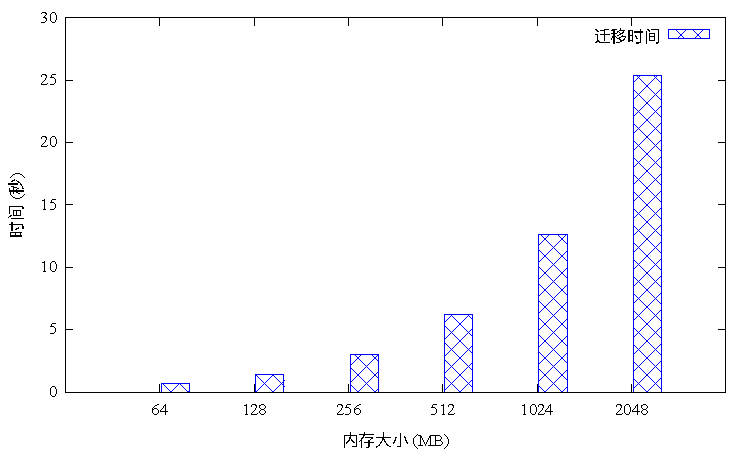
\includegraphics[width=1.0\textwidth]{migrationtime}
  \caption{活迁移时间开销}
  \label{figure:migrationtime}
\end{figure}

因为m3.large类型实例的全部内存是7.5 GB,在这个类型的竞价虚拟机实例上的所有在线服务在两分钟的回收告警时间内肯定可以完成进程活迁移。对于其他类型的内存更大的虚拟机实例,网络带宽也提升到了1 Gbps,甚至对于一些超大型(Extra Large)虚拟机实例网络带宽达到了10 Gbps。因此,可以肯定的是Gemini采用进程活迁移的方式保证在竞价实例回收风险下的服务可用性是可行的。此外,使用进程活迁移的手段避免了进行内存检查点操作带来的性能开销。

\subsubsection{I/O性能}
Gemini和一些其他配置下的I/O性能对比是本节的测试目标。这个测试使用了Linux m3.large型计算实例。Linux m3.large型虚拟机实例的本地实例存储是一个32 GB的SSD卷。Gemini使用一个同为32 GB大小的通用型(General Purpose)SSD EBS作为后端存储设备。通用型SSD EBS可以持续提供 3 IOPS/GB 的基准性能,并支持突发性的I/O请求能提供高达3000 IOPS的性能。实验中使用fio \cite{FIO:2014},一个灵活的I/O测试集工具,来对比Gemini的时间可控异步磁盘同步配置,通常的同步磁盘镜像配置,和其他两个存储配置,裸SSD实例存储和裸通用型SSD EBS。测试读写用文件2 GB大小,测试使用8个进程提交16 KB大小的顺序和随机I/O请求。I/O请求队列深度为64,测试时间为60秒。由于实例存储和EBS卷都是虚拟的,每个磁盘块第一个访问时可能有5\%到50\%的性能损失,实验前对待测的存储设备进行了预热处理。
\begin{figure}[]
  \centering
  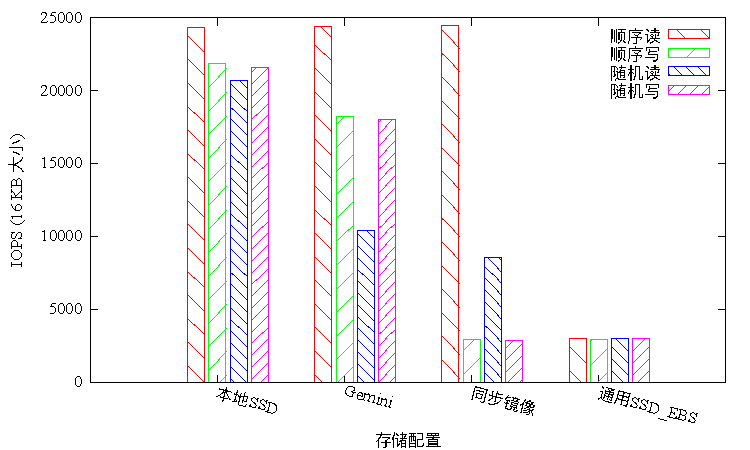
\includegraphics[width=1.0\textwidth]{iops}
  \caption{不同存储配置下的IOPS}
  \label{figure:iops}
\end{figure}

图 \ref{figure:iops} 显示了不同存储配置下的IOPS。毫无疑问,非持久化的SSD实例存储拥有最好的I/O性能。SSD实例存储可以提供高达20000 IOPS的性能,无论是顺序还是随机,读还是写测试。通用型SSD EBS的突发I/O性能在四个测试中的可达到约3000 IOPS。这仍要比SSD实例存储慢7倍左右。对于SSD实例存储和通用型SSD EBS设置为同步镜像的配置,写性能被限制在通用型SSD EBS的IOPS水平。顺序写之后的顺序读性能同SSD实例存储类似,约25000 IOPS。随机读测试性能适中,因为读请求部分由SSD实例存储响应,未缓存的部分则由通用型SSD EBS处理。Gemini的时间可控异步磁盘镜像机制相比同步镜像有更好的性能。其顺序和随机写性能接近SSD实例存储,顺序读性能也接近25000 IOPS。

\subsection{服务性能}
这里选择了两个基准测试集,TPC-W 和 YCSB 用于测试在线服务在Gemini框架下的性能。TPC-W 是一个模拟网上书店的交易事务测试集。YCSB 可以生成各种NoSQL数据库的工作负载。这里使用YCSB评测SSD实例存储可以多大程度上提升MongoDB的性能。

\subsubsection{TPC-W 基准测试}
TPC-W 是一个计算密集的基准测试集。这个测试主要比较Gemini的轻量级服务迁移方案和基于嵌套虚拟化和虚拟机迁移技术的方案在性能开销上的表现。这里选取了一个Java Servlets版本的TPC-W实现 \cite{JAVATPCW:2014}。其中,web应用前端部署在Apache Tomcat 7上,数据库后端使用的是MySQL 5.0。Web服务器和数据库服务器运行在Linux m3.large类型虚拟机实例上,主要配置为2 VCPUs 和 7.5 GB 内存。测试中使用另外的虚拟机实例生成模拟浏览器(Emulated Browsers)作为访问用户。测试中使用混合订单型(Ordering Mix)负载,其中有50\% 为浏览交互,50\%为下订单交互。

用于比较,在Linux m3.large上运行的Xen-Blanket \cite{Williams:2012:XVO:2168836.2168849} 嵌套虚拟机管理器创建了一个嵌套虚拟机。它的配置为2 VCPUs 和 7 GB内存,因为虚拟机管理器也需要使用一部分内存。这并不会带来性能差异,因为Tomcat和MySQL测试中使用的内存量远远小于7 GB。

图 \ref{figure:tpcw} 显示了在不同用户请求压力下web交互的平均响应时间。Gemini的表现从50个到400个模拟浏览器一直好于基于嵌套虚拟化的解决方案。Gemini的性能开销接近于0,因为在服务正常运行时没有内存检查点任务。而基于嵌套虚拟化的方法在运行TPC-W基准测试集时则出现了的30\% 到 45\%性能开销。
\begin{figure}[]
  \centering
  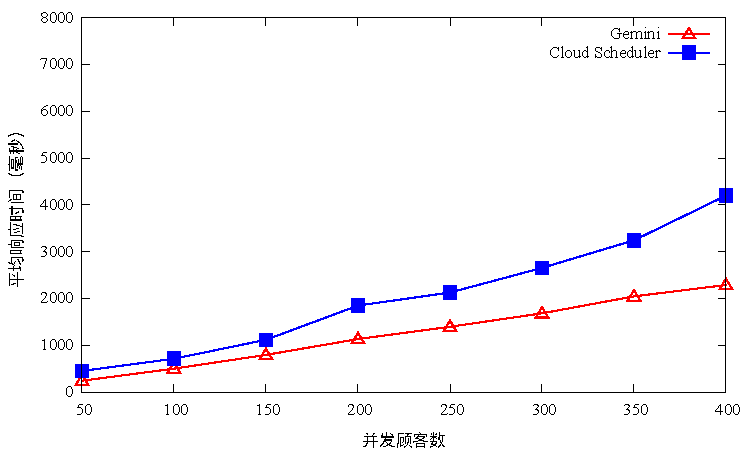
\includegraphics[width=1.0\textwidth]{tpcw}
  \caption{TPC-W测试集中不同请求压力下的平均响应时间}
  \label{figure:tpcw}
\end{figure}

对于计算密集的工作负载,如此大的性能开销意味着为提升性能到原来的水平必须在使用一个虚拟机实例。使用轻量级的进程迁移技术显然是一个更好的选择。此外,Gemini使用的基于暖备的故障转移方式消除了申请新的虚拟机实例所需的时间。Gemini可以将全部两分钟回收告警时间用于服务迁移,包括同步磁盘镜像和进程迁移。当活迁移可以安全地在告警时间内完成,内存检查点就没有必要了。这进一步减少了性能开销。

\subsubsection{YCSB 负载测试集}
我们选择了两个典型的YCSB负载测试MongoDB的性能。一个是更新较多的负载,有 50\% 的读操作和 50\% 的更新操作。另一个是读为主的负载,有 95\% 的读操作和 5\% 的更新操作。所有请求在数据库的键名空间呈正态分布。实验仍然在Linux m3.large类型的虚拟机实例上进行,这个类型的节点有32 GB的SSD实例存储。一个同样32 GB大小的通用型SSD EBS用于备份存储。Gemini以时间可控的方式复制SSD实例存储的磁盘更新到SSD EBS。在Gemini配置下和通用型SSD EBS下的吞吐和延迟数据如图 \ref{figure:ycsba} 和图 \ref{figure:ycsbb} 所示。

Gemini在更新频繁的负载下可以达到通用型SSD EBS约两倍的吞吐。在两个负载下,Gemini的读延迟和通用型SSD EBS几乎相同。Gemini大幅减少了写延迟,在更新频繁的负载压力下写延迟相比通用型SSD EBS的性能改善有约2.5倍之多。如图\ref{figure:ycsbb}所示,对于以读为主的负载,Gemini只有相对SSD EBS至多 18\% 的吞吐性能提升。因此MongoDB对大部分读请求的处理有效利用了内存中的缓存数据。

\begin{figure}[]
  \centering
  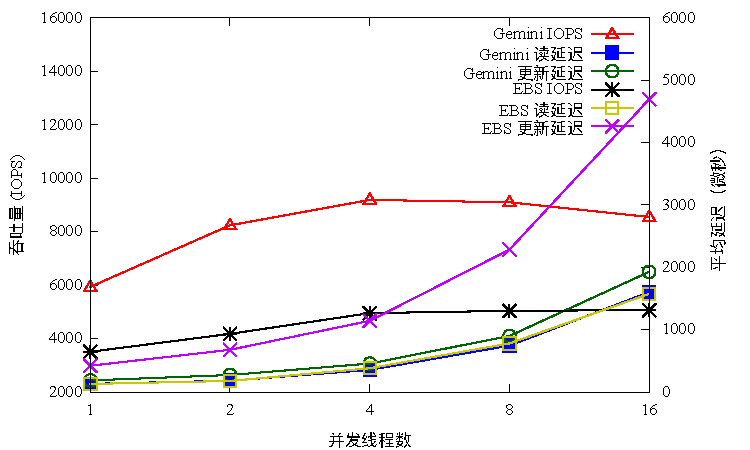
\includegraphics[width=1.0\textwidth]{ycsba}
  \caption{MongoDB在更新频繁负载下的吞吐性能}
  \label{figure:ycsba}
\end{figure}

\begin{figure}[]
  \centering
  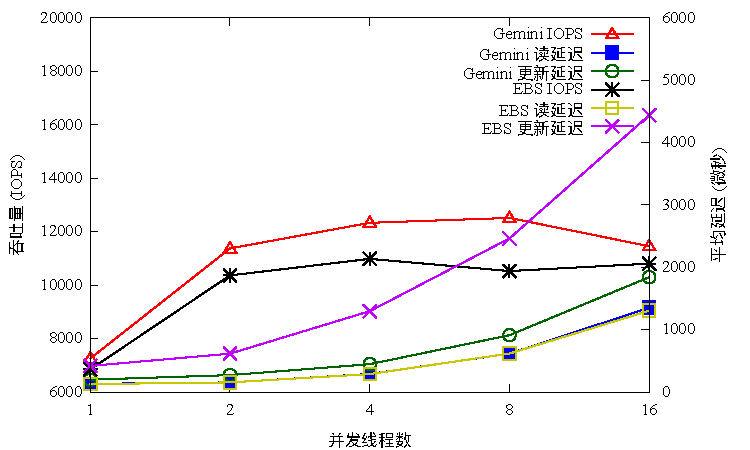
\includegraphics[width=1.0\textwidth]{ycsbb}
  \caption{MongoDB在以读为主负载下的吞吐性能}
  \label{figure:ycsbb}
\end{figure}

\subsection{成本与可用性分析}
根据虚拟机实例的获取时间,服务迁移时间,以及Amazon EC2的竞价实例市场价格历史数据,本节进行了一个长期(约1个月时间)的在线服务运行仿真。仿真参数包括虚拟机实例获取时间和服务迁移时间等,保证了仿真结果的有效性。按需实例和竞价实例的启动时间数据由 Mao 等人 \cite{Mao:2012:PSV:2353730.2353859} 收集。不同内存大小的进程迁移时间已在 \ref{sec-migrationtime} 小节中作为一个指标测量过。

仿真中的在线服务为TPC-W基准测试集中的网上书店。网上书店的架构包括一个WEB服务器和一个数据库服务器,各使用一个虚拟机实例。在Gemini中,这两个节点被迁移控制器组织成一个暖备对。这是一个Gemini框架下最小的常用案例。实验中分别使用小型、中型、大型、超大型虚拟机实例进行这样一个在线服务的仿真。通过这些仿真,使用Gemini在竞价云平台上提供在线服务的成本和可用性得以评测。使用暖备配置和冷备配置,以及不同可用区选择策略的比较可以得出。

因为虚拟机实例调度器根据近期竞价实例市场价格数据的标准差(Standard Deviation)和简单移动平均值(Simple Moving Average)选择可用区,这个选择策略被表示为``SD-SMA''。另一个简单的策略是选择当前竞价实例市场价格最便宜的可用区,可以表示为``Greedy''。在Gemini中,竞价价格被设置为相应按需实例的价格。因为当竞价实例市场价高于按需实例价格时,应该选择使用按需实例。基于冷备的框架,像Cloud Scheduler,设置了一个高于按需实例价格的竞价以减少过多的强制性迁移。但这对于竞价实例市场价格的剧烈抖动是无效的。将可用区选择策略和故障转移机制组合到一起有四种选择:``Cold Greedy'',``Warm Greedy'',``Cold SD-SMA'',``Warm SD-SMA''。其中 ``Cold Greedy'' 是 Cloud Scheduler 的选择,``Warm SD-SMA'' 是Gemini的选择。

仿真测试中四种选择下的服务不可用性如图 \ref{figure:cost} 所示,基于暖备对的解决方案的服务可用性在小型、中型、大型、超大型虚拟机实例下都比基于冷备的框架好多达一个数量级。因为在Gemini的HA配置中,在线服务只有在活迁移过程中的冻结时间处于不可用状态。通过使用Pre-copy迁移方式,冻结时间可以降低到数十毫秒。而且活迁移可以在收到回收告警后立即开始。然而,基于冷备的框架在强制性迁移时必须首先获取一个新的虚拟机实例。虚拟机实例的启动时间严重影响了在线服务在这一场景下的可用性。设置一个比按需实例价格更高的竞价在超大型虚拟机实例的案例下取得了较好的效果。因为这一类型的虚拟机实例经常波动到超过按需实例价格的程度。
\begin{figure}[]
  \centering
  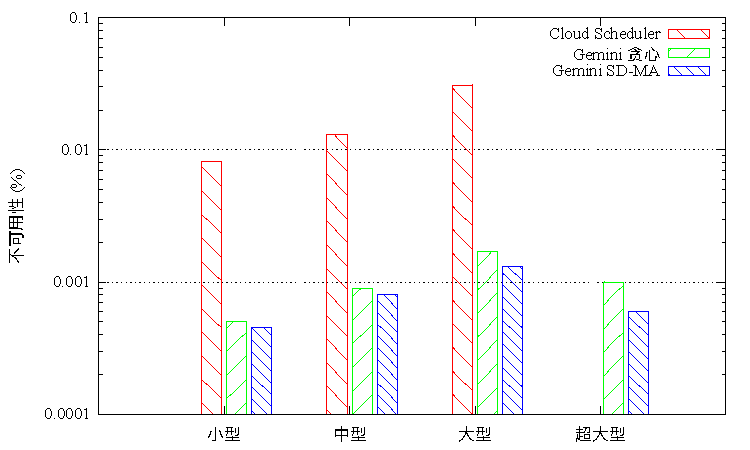
\includegraphics[width=1.0\textwidth]{availability}
  \caption{单区域不可用性比较}
  \label{figure:unavailability}
\end{figure}

无论是一个基于冷备的框架,还是Gemini,``SD-SMA''的策略相比``Greedy''的策略减少了强制性迁移的次数。这一策略在大多数情况下通过选择价格稳定的可用区取得了更好的可用性。相对地,如图 \ref{figure:cost} 所示这个策略在一些情况下成本更高。这是因为最便宜的可用区有时不够稳定。图 \ref{figure:cost}显示了在 ``us-west2'' 区域使用不同框架提供在线服务的归一化成本。基线是使用按需实例提供这一在线服务的成本。Gemini的成本大致只有基线的 14\% 到 23\%。这同 Cloud Scheduler 接近。
\begin{figure}[]
  \centering
  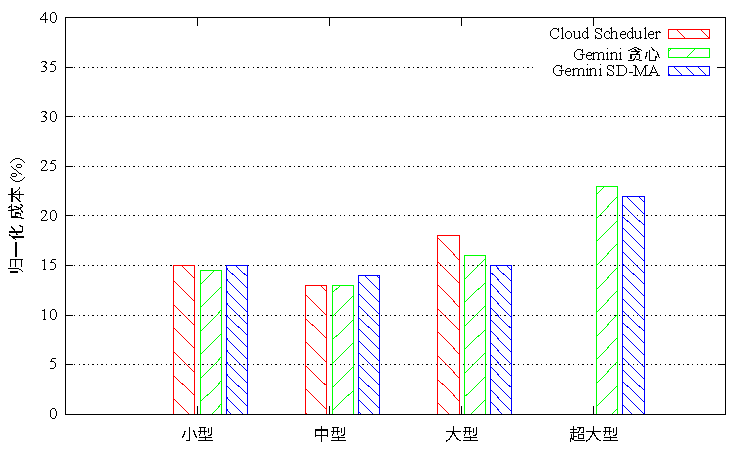
\includegraphics[width=1.0\textwidth]{cost}
  \caption{单区域的成本比较}
  \label{figure:cost}
\end{figure}

实验还进行了多区域场景下的仿真。只有美国的三个区域:``us-west1'',``us-west2'',``us-east''在实验中被使用。图 \ref{figure:unavailabilitymulti} and \ref{figure:costmulti} 显示了在多个区域中利用Gemini等框架提供在线服务的成本和可用性情况。Gemini的可用性相比单区域情况有所提升。因为有更多的可用区作为候选可以使在线服务运行在竞价实例价格更稳定的可用区上。然而,多区域下``Greedy''策略在某些情况下的不可用性有所增加。这是由于便宜的可用区可能价格不稳定,这导致在多个区域中贪心地选择最便宜的可用区可能经历更多的强制迁移。
\begin{figure}[]
  \centering
  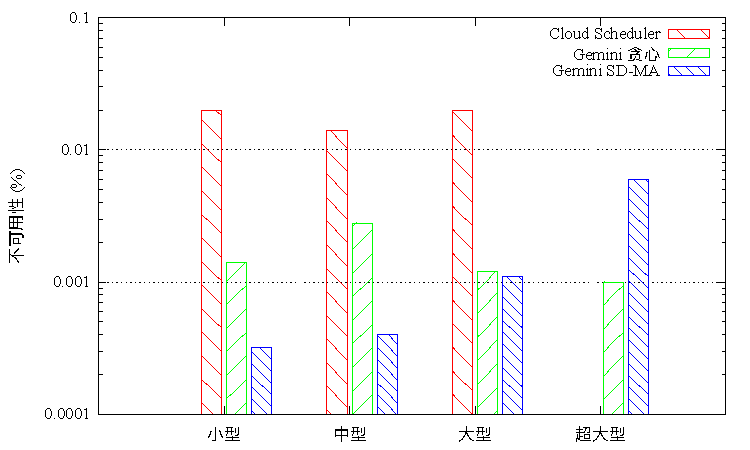
\includegraphics[width=1.0\textwidth]{availabilitymulti}
  \caption{多区域不可用性比较}
  \label{figure:unavailabilitymulti}
\end{figure}

如图所示,在多区域下提供在线服务的成本效率在大多数情况下得以改善。Gemini的成本在几种不同的实例类型下低至基线的 11\% 到 22\%。使用 ``SD-SMA'' 策略的成本略高于 ``Greedy'' 策略,但获得了显著的可用性提升。
\begin{figure}[]
  \centering
  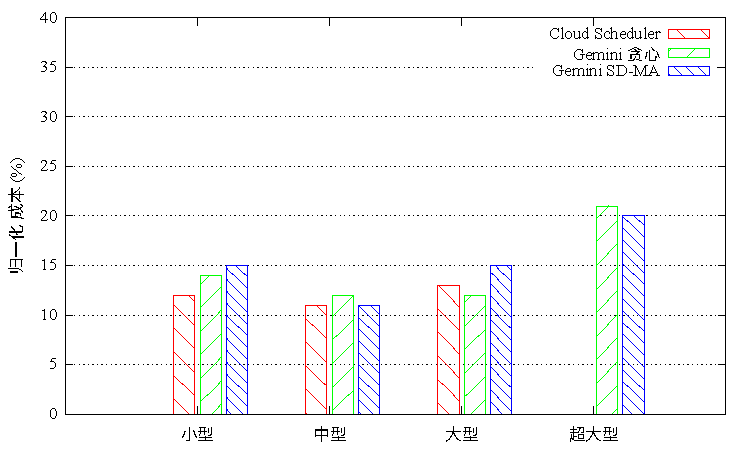
\includegraphics[width=1.0\textwidth]{costmulti}
  \caption{多区域的成本比较}
  \label{figure:costmulti}
\end{figure}

\section{本章小节}
Gemini提供了一个轻量级的使用竞价实例运行在线服务的高可用方案。同已有方案相比,Gemini通过基于暖备的故障转移方式消除了强制性不可用的情况。而且Gemini使用轻量级的进程活迁移机制减少了服务运行和迁移过程中的性能开销。出于性能方面的考虑,在Gemini的设计中允许在线服务使用高性能的SSD实例存储。Gemini负责从SSD实例存储复制数据更新到网络上的EBS以实现数据持久化。为保证可以在回收告警时间内完成同步同时提供最好的I/O性能,Gemini使用了时间可控的异步磁盘镜像机制。通过组合几个系统级技术,Gemini提供了在不可靠的竞价实例上运行在线服务的故障转移机制。当互备对中的一个节点被云平台回收时,Gemini通过备用节点保证可用性,同时从云平台获取一个虚拟机实例以恢复原来的高可用配置。在Gemini原型系统上的一系列的实验验证和评测了这一解决方案的有效性。在TPC-W基准测试集下,Gemini 相比基于嵌套虚拟化的解决方案可以减少 30\% 到 45\% 的性能开销。在 YCBS 更新频繁的负载下,Gemini 框架下的 MongoDB 可以获得大约两倍的吞吐性能提升和 2.5 倍的写延迟性能提升。基于 Amazon EC2 平台 已公布的竞价实例历史价格数据的长期在线服务仿真显示:Gemini相比之前的解决方案在可用性上实现了一个量级的提升,以及相比使用按需实例五到六倍的成本节省(和已有方案相近)。